\documentclass{article}
\usepackage{booktabs}
\usepackage{graphicx}

\title{Biol 461 Winter 2021 Assignment 2}
\author{Due 11:59pm January 22 2021}
\date{}

\begin{document}

\maketitle

\subsection*{Instructions}
This assignment is broken into three parts. Part one consists of questions drawn from the lectures and readings assigned thus far in the course. There are X number of points available for part 1. Part two consists of questions concerning the Moreno 2016 paper. There are x number of points available for part 2. For part three, choose and complete \textbf{one} of the two provided options.\\\\
Please submit by uploading a PDF copy of your solutions to the Canvas assignment. Failure to submit the homework in the correct way and in the correct format may result in deduction of points. Incorrect solutions that do not show work will not receive any partial credit, so show your work where appropriate. \\\\
Collaboration with classmates is encouraged; however, your solutions should reflect your own understanding and all explanations should be in your own words. Please make a note of who you worked with.

\subsection*{Part 1}

\subsection*{Problem 1 (X pts)}
In lecture we learned that the longest cell in the human body is a sensory neuron from the dorsal root ganglion of the spine. It stretches from the tip of your toes the the bottom part of your brain. Calculate how long it would take an action potential to propagate from one end of this neuron to the other if the neuron is 1.6 meters long.

\pagebreak{}
\subsection*{Problem 2 (X pts)}
\begin{enumerate}
    \item[A.] If you exposed a neuron to a drug that blocked all voltage gated sodium channels, what would happen to the waveform of the action potential? Draw what the waveform would like look superimposed on the control action potential drawing below.\\\\
    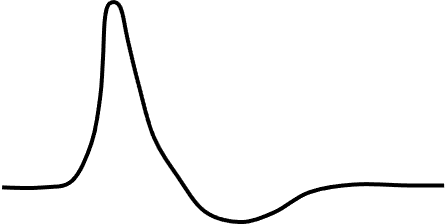
\includegraphics[scale = 1]{action_potential.png}
    \item[B.] If you exposed a neuron to a drug that blocked all voltage gated potassium channels, what would happen to the waveform of the action potential? Draw what the waveform would like look superimposed on the control action potential drawing below.\\\\
    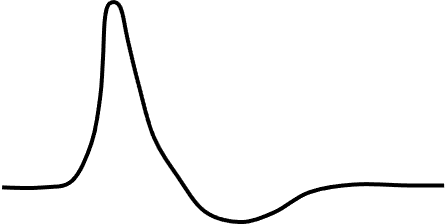
\includegraphics[scale = 1]{action_potential.png}
\end{enumerate}

\subsection*{Problem 3 (X pts)}
Name 2 different mechanisms by which the strength of a synapse might change (synaptic plasticity) and explain how this mechanism may lead to a stronger or weaker synapse (1--2 sentences each).

\pagebreak{}
\subsection*{Problem 4 (x pts)}
For each labeled point (A–D) on the action potential shown in Figure Q2–34, state whether the conductance through voltage-dependent Na+ and K+ channels is low, high, or no conductance. Explain. [Note: For this answer, ignore conductance through leak channels.]\\\\
\begin{center}
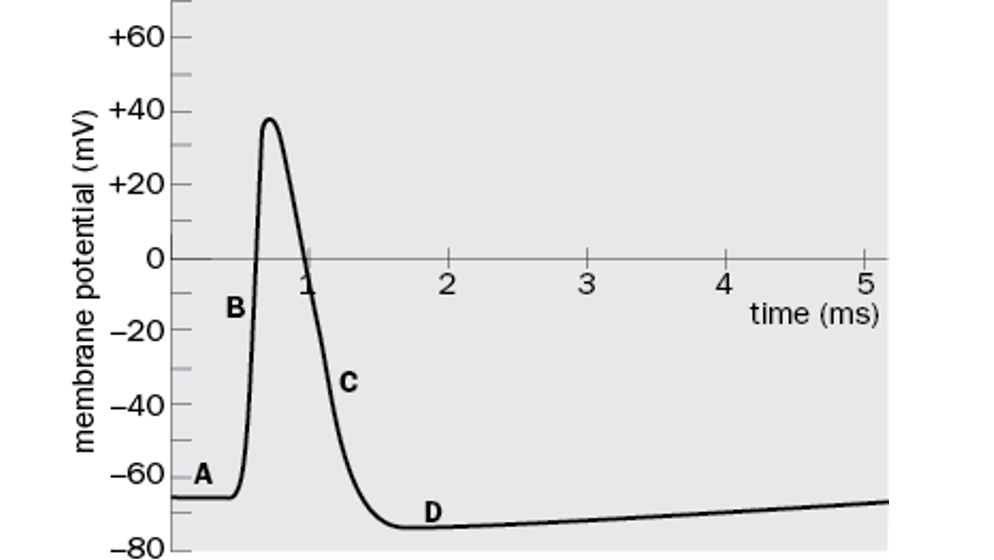
\includegraphics[scale = .8]{action_potential_with_axis.png}\\
\end{center}
\\
A.\\\\\\\\\\
B.\\\\\\\\\\
C.\\\\\\\\\\
D.

\subsection*{Part 2}
1. Summarize Major Points\\
2. Why are these findings important?\\
3. What was the experimental approach? What type(s) of experiment(s) did they do?\\
4. Where in the paper do the authors support the claim .......... What data do they use to support this claim?

\subsection*{Part C}
Choose EITHER

1. Use the Hodgens/Huxley model equations to derive the action potential\\
2. Read this biochem paper that goes in depth about the voltage-sensitive part of an ion channel\\
3. Read this paper about neurons releasing multiple neurotransmitters?
\end{document}
